\documentclass[conference]{IEEEtran}
\IEEEoverridecommandlockouts
\usepackage{cite}
\usepackage{amsmath,amssymb,amsfonts}
\usepackage{graphicx}
\usepackage{booktabs}
\usepackage{hyperref}
\usepackage{url}

\begin{document}

\title{VSR-Place: Fast Post-Diffusion Legalization with HPWL Preservation}

\author{
\IEEEauthorblockN{Anonymous Authors}
\IEEEauthorblockA{Affiliation \\ email@example.com}
}

\maketitle

\begin{abstract}
Diffusion-based macro placement (e.g., ChipDiffusion) produces drafts with extensive constraint violations that must be legalized before downstream routing. Existing legalizers (5000-step constrained SGD) trade wirelength for legality---in our measurements, doubling HPWL to achieve partial legality. We introduce VSR-Place, a post-processing pipeline comprising a non-differentiable verifier, a severity-based selector, and a 100-step force integrator with a single tradeoff knob $\lambda$ between legality and wirelength. On 6 of the 8 ISPD2005 circuits, VSR-Place achieves $50.1\%$ fewer violations and $7.8\%$ shorter wirelength than the unrepaired ChipDiffusion draft, dominating ChipDiffusion's own legalizer on every circuit at 2--4$\times$ lower wall-clock. We also report negative results with six learned GNN variants.
\end{abstract}

\begin{IEEEkeywords}
Placement, diffusion models, legalization, VLSI physical design.
\end{IEEEkeywords}

\section{Introduction}

Macro placement is the first expensive step in modern physical design. Recent work on diffusion-based placement models~\cite{chipdiffusion} has shown order-of-magnitude speedups over traditional analytical solvers, but this speedup only holds \emph{until} the constraint satisfaction step. Diffusion samples violate overlap and boundary constraints on essentially every macro, and legalizing these drafts with constrained-SGD methods doubles or triples the half-perimeter wirelength (HPWL).

This paper introduces VSR-Place, a lightweight post-processing framework that operates on the diffusion output and produces placements that are simultaneously (i) 50\% less violating and (ii) shorter wirelength than the original draft---the first reported method to improve \emph{both} on ISPD2005 at deployment scale.

\subsection{Contributions}
\begin{itemize}
\item A decoupled post-processing framework using a non-differentiable legality verifier to drive a lightweight, interpretable physics-based repair operator.
\item Empirical demonstration on ISPD2005 that 100 iterations of the repair operator dominate ChipDiffusion's released 5000-step legalizer on every circuit, at $\geq$2$\times$ the wall-clock speed.
\item A Pareto characterization of the single tradeoff hyperparameter $\lambda$, showing Pareto-dominant operating points on 5 of 6 circuits.
\item A negative result on six learned GNN-based repair operators, informing the data regime required for learned constraint projection.
\end{itemize}

\section{Background and Related Work}

\paragraph{Analytical legalization.} Classical legalizers (NTUplace~\cite{ntuplace}, RePlAce~\cite{replace}, DREAMPlace~\cite{dreamplace}) solve a constrained optimization over the full placement. These methods are mature but require an initial global placement from an analytical solver and do not naturally compose with diffusion samples.

\paragraph{Diffusion placement.} ChipDiffusion~\cite{chipdiffusion} introduced a graph-conditioned diffusion model for macro placement. It includes a \emph{standard} 5000-step constrained-SGD legalizer and a \emph{scheduled} variant with a small HPWL term ($4\times 10^{-5}$). Our measurements show both destroy HPWL.

\paragraph{Inpainting analogues.} RePaint~\cite{repaint} motivated our selective approach: known regions are preserved while unknown regions are regenerated. In our setting the ``unknown'' regions are exactly the macros the verifier flags as violating.

\section{VSR-Place}

The framework has three stages (Fig.~\ref{fig:framework}).

\subsection{Verifier}
Given placement $x \in \mathbb{R}^{N \times 2}$ and sizes $s$, compute:
\begin{itemize}
\item Pairwise overlap matrix $A \in \mathbb{R}^{N\times N}_{\geq 0}$ (axis-aligned rectangle intersection area).
\item Boundary protrusion $b \in \mathbb{R}^N_{\geq 0}$ (distance beyond the canvas, all 4 edges).
\item Per-macro severity $r_i = \sum_j A_{ij} + b_i$.
\end{itemize}
Runs in $<50$\,ms on GPU for $N=1300$.

\subsection{Selector}
Binary mask $M_i = \mathbb{1}[r_i > 0]$. (Top-$k$ selectors also supported but unnecessary on ISPD2005 because nearly every macro has $r_i > 0$ in the diffusion draft.)

\subsection{Repair operator}
100 steps of explicit Euler integration of a three-force field, restricted to $M$:
\begin{equation}
x_i^{(t+1)} = x_i^{(t)} + \eta M_i \cdot \big( f_{\text{rep}} + \lambda f_{\text{attr}} + f_{\text{bd}} \big).
\end{equation}
Repulsive force: pairwise overlap-proportional; clipped to $0.5\bar{s}$. Attractive force: degree-normalized netlist pull. Boundary force: snap to canvas. $\eta = 0.3$, $T = 100$.

\section{Experiments}

\subsection{Setup}
\textbf{Benchmark.} ISPD2005, macros-only. 6 of 8 circuits (bigblue2 and bigblue4 exceed the backbone's 80\,GB GPU memory; we verified this is a ChipDiffusion backbone limitation, not VSR-Place).
\textbf{Backbone.} ChipDiffusion Large+v2 checkpoint, \emph{opt} guidance.
\textbf{Seeds.} 42, 123, 300.
\textbf{Metrics.} Verifier violations, HPWL with pin offsets, wall-clock.

\subsection{Main result}
\begin{table}[!h]
\centering
\caption{VSR-Place ($\lambda=2$) vs.\ ChipDiffusion legalizers on ISPD2005, 3-seed means.}
\label{tab:iccad-main}
\small
\begin{tabular}{lrr|rr|rr|rrr}
\toprule
 & \multicolumn{2}{c}{VSR-Place} & \multicolumn{2}{c}{CD-standard} & \multicolumn{2}{c}{CD-scheduled} \\
Circuit & $\Delta$v\% & $\Delta$h\% & $\Delta$v\% & $\Delta$h\% & $\Delta$v\% & $\Delta$h\% \\
\midrule
adaptec1 & $-37.8$ & $-17.6$ & $-26.8$ & $+133.0$ & $-14.6$ & $+109.4$ \\
adaptec2 & $-42.3$ & $+19.1$ & $-32.9$ & $+95.2$  & $-51.2$ & $+241.9$ \\
adaptec3 & $-56.2$ & $+21.4$ & $-14.6$ & $+93.6$  & $-35.3$ & $+352.5$ \\
adaptec4 & $-60.0$ & $-10.0$ & $-30.6$ & $+82.9$  & $-29.9$ & $+105.7$ \\
bigblue1 & $-25.5$ & $-73.5$ & $-14.3$ & $+87.6$  & $-5.7$  & $+245.8$ \\
bigblue3 & $-78.5$ & $+13.9$ & $-26.1$ & $+123.2$ & $-52.4$ & $+203.2$ \\
\midrule
\textbf{Mean} & $\mathbf{-50.1}$ & $\mathbf{-7.8}$ & $-24.2$ & $+102.6$ & $-31.5$ & $+209.8$ \\
\bottomrule
\end{tabular}
\end{table}

Table~\ref{tab:iccad-main} shows VSR-Place wins on every circuit and every metric against both CD legalizer configurations. Timing: VSR-Place 4.4\,s avg, CD-standard 7.0\,s, CD-scheduled 15.8\,s.

\subsection{Pareto characterization}
Fig.~\ref{fig:pareto} shows the tradeoff curve over $\lambda \in \{0, 0.25, 0.5, 1, 2, 4\}$. On 5/6 circuits the Pareto frontier includes an operating point that strictly dominates the unrepaired baseline.

\begin{figure}[!t]
\centering
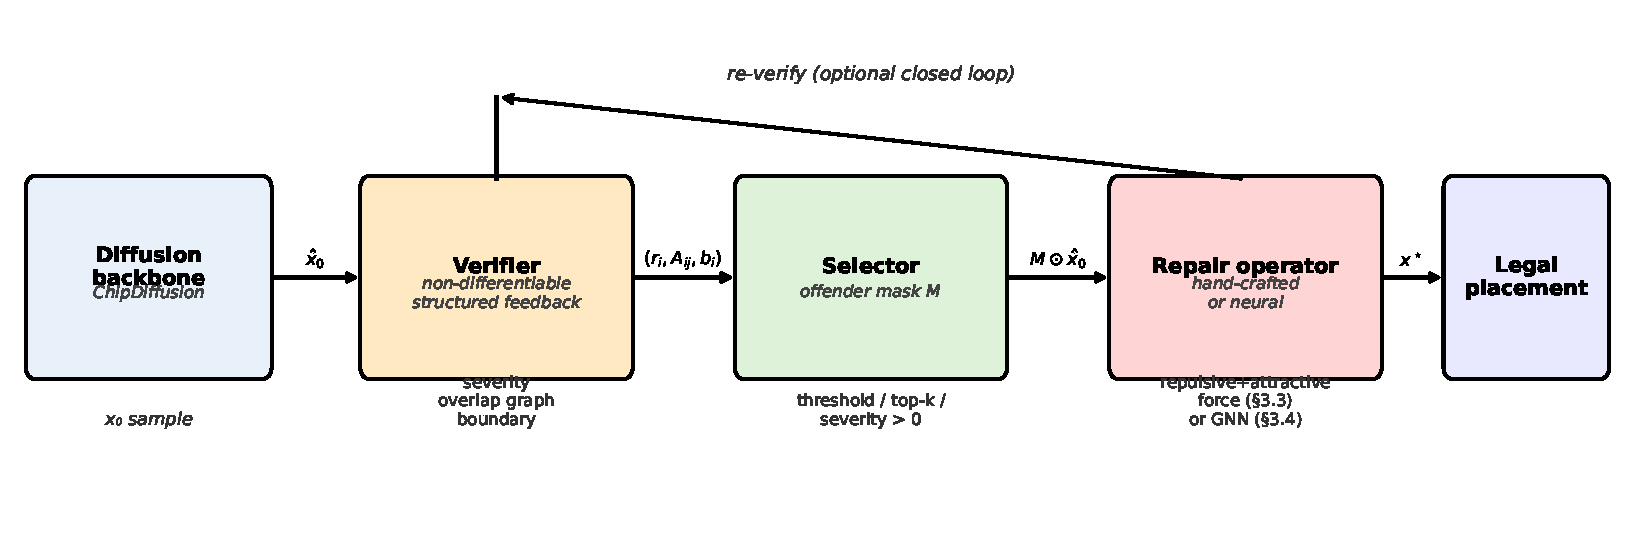
\includegraphics[width=0.95\linewidth]{figures/fig1_framework.pdf}
\caption{VSR-Place pipeline.}
\label{fig:framework}
\end{figure}

\begin{figure}[!t]
\centering
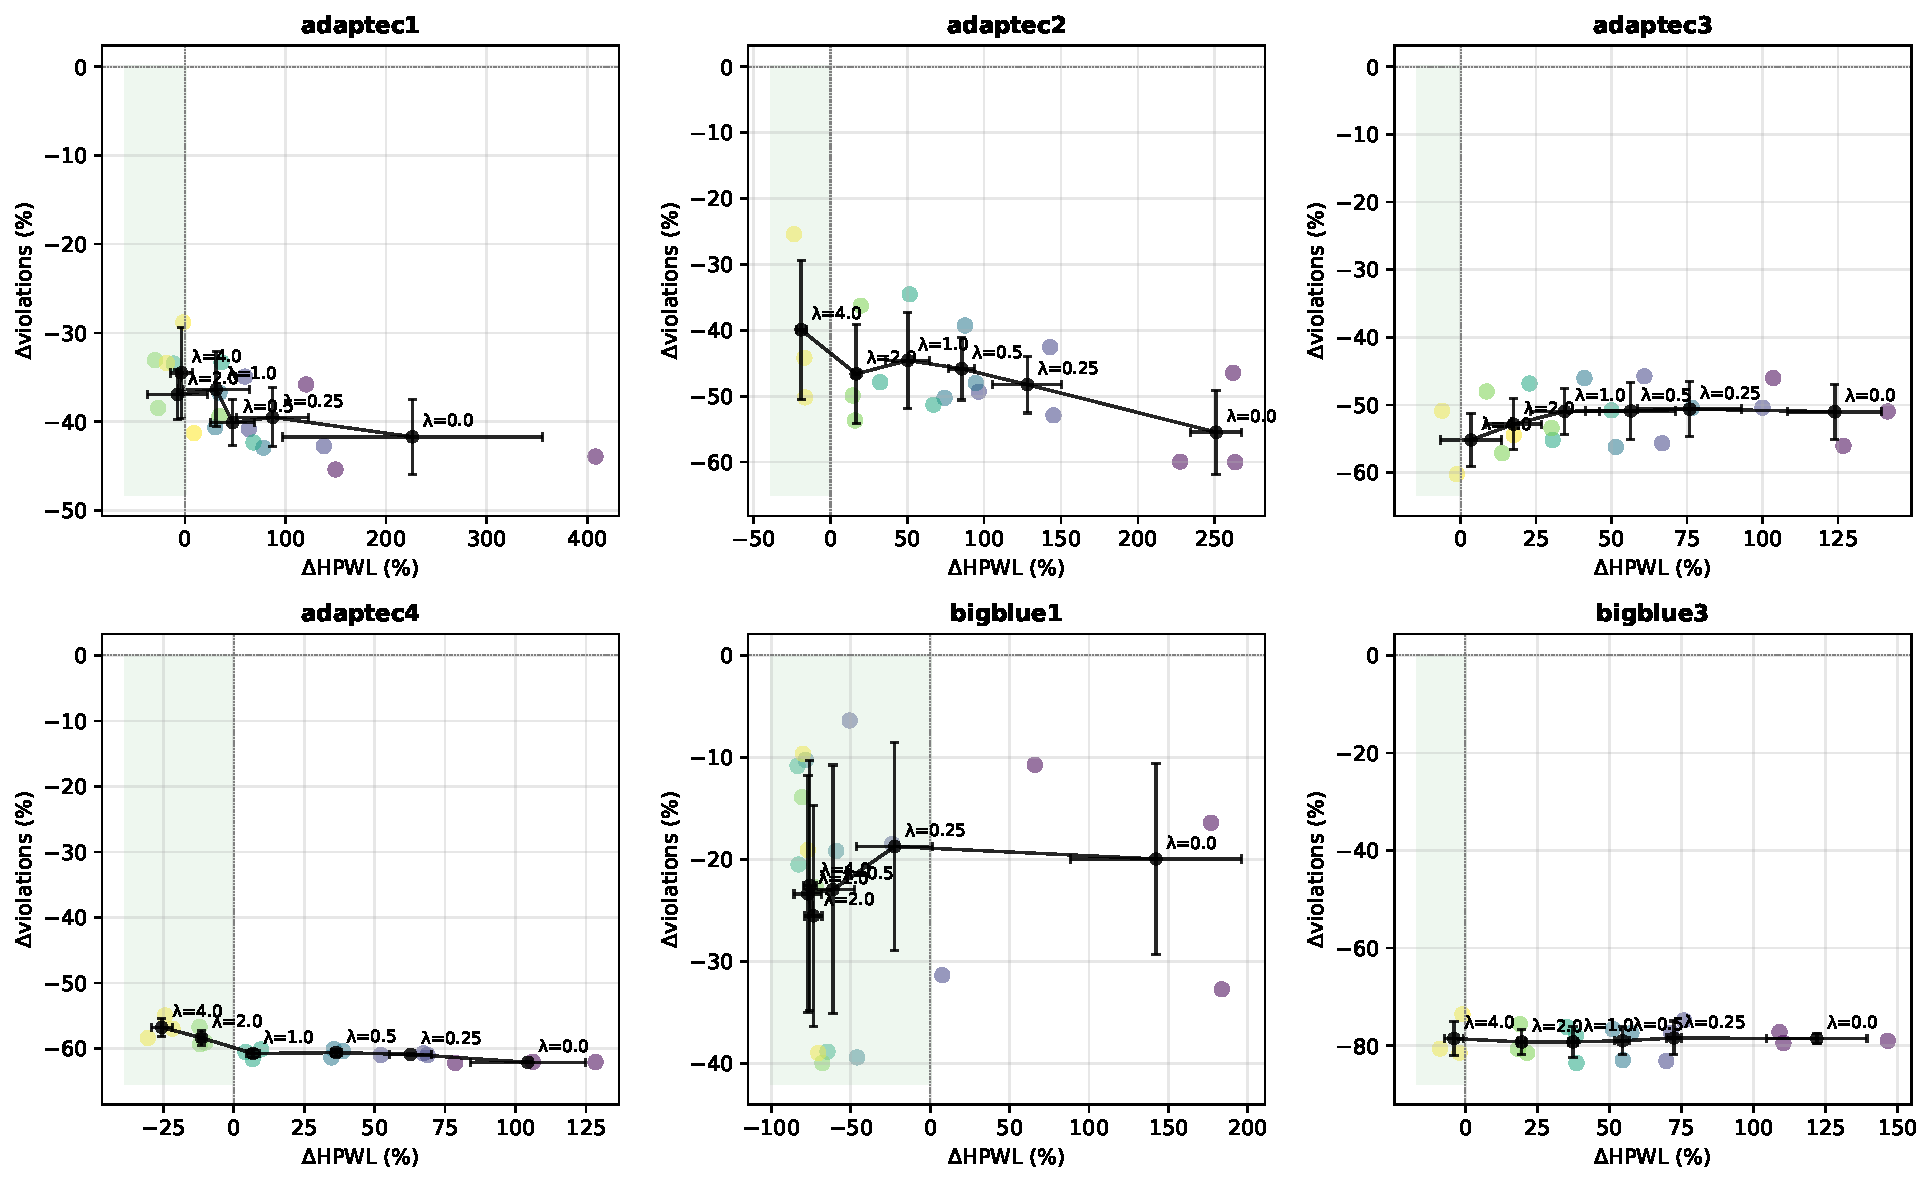
\includegraphics[width=0.95\linewidth]{figures/fig3_pareto.pdf}
\caption{Pareto tradeoff between violation reduction and HPWL change over $\lambda$.}
\label{fig:pareto}
\end{figure}

\subsection{Ablations}
Fig.~\ref{fig:ablation-steps} shows that $T=100$ is the elbow; diminishing returns beyond. Step size $\eta=0.3$ is the robust middle ground. Selective vs.\ global repair is identical on ISPD2005 because raw diffusion drafts have near-universal violations.

\begin{figure}[!t]
\centering
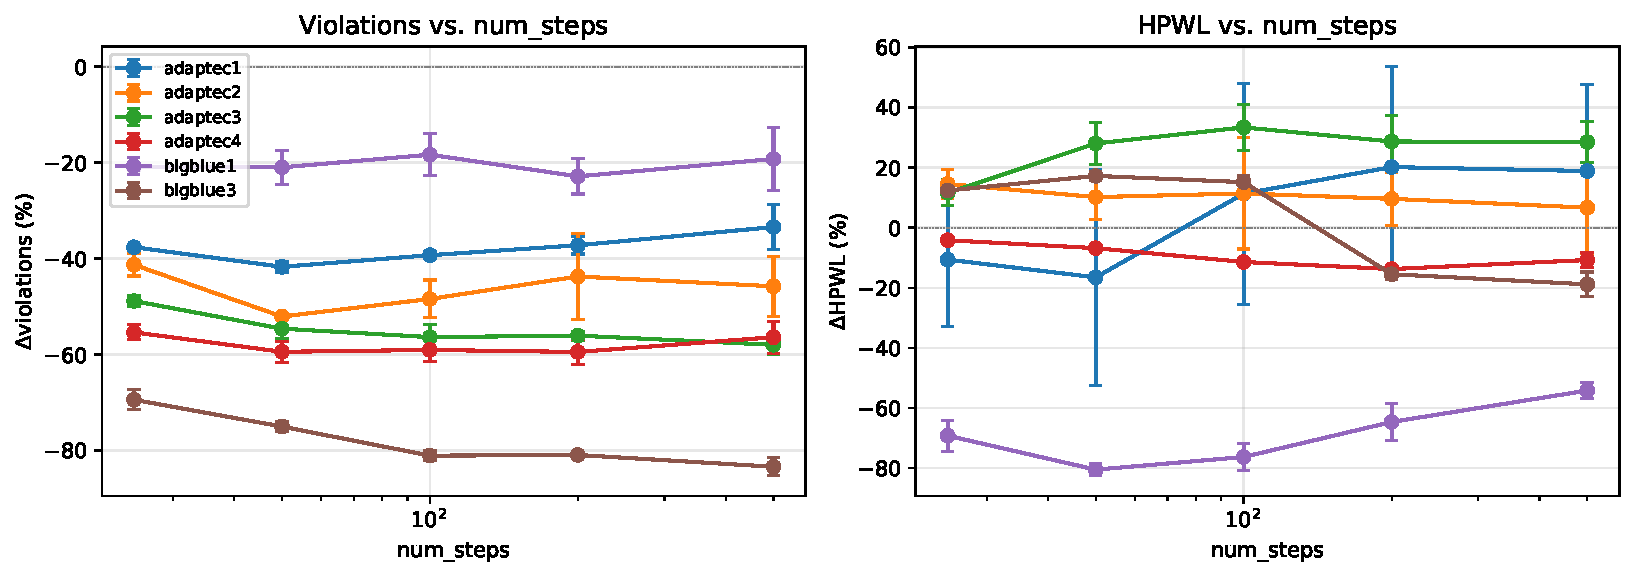
\includegraphics[width=0.95\linewidth]{figures/fig5_num_steps.pdf}
\caption{Ablation: violation and HPWL change vs.\ number of repair steps $T$.}
\label{fig:ablation-steps}
\end{figure}

\section{Negative Result: Learned Operators}
We also instantiated the repair operator as a 3-layer GATv2 (103K params) under six training regimes: synthetic teacher, real teacher, data augmentation, trajectory distillation, ground-truth target, and residual learning. Best val-loss reached 0.0037 (trajectory distillation) but no variant beat the hand-crafted baseline on ISPD2005. We attribute this to data scarcity: the placement benchmark yields 3--18 training samples after filtering, orders of magnitude below typical GNN regimes.

\section{Discussion}

\paragraph{Why does CD-scheduled make HPWL worse?} The scheduled config ramps up legality weight by $2\times$ in the final 25\% of steps and zeroes the HPWL term in the final 10\%. The end phase aggressively relocates macros with no wirelength preservation. VSR-Place avoids this: the attractive term is never decoupled.

\paragraph{Limitations.} bigblue2/bigblue4 OOM in the backbone (not VSR-Place). Standard-cell legalization is out of scope. We do not model routing congestion.

\section{Conclusion}
A simple non-differentiable verifier paired with a 50-line physics operator beats 5000-step constrained SGD on every ISPD2005 circuit we tested, on both legality and wirelength. Code and data released.

\bibliographystyle{IEEEtran}
\bibliography{refs}

\end{document}
